\documentclass[times, utf8, zavrsni]{fer}
\usepackage{booktabs}
\usepackage[hyphenbreaks]{breakurl}
\usepackage{gensymb}

\begin{document}

\thesisnumber{7031}

\title{Višedretvena izvedba algoritma računanja histograma orijentacija gradijenata u slikama}

\author{Mateo Imbrišak}

\maketitle

% Dodavanje zahvale ili prazne stranice. Ako ne želite dodati zahvalu, naredbu ostavite radi prazne stranice.
\zahvala{}

\tableofcontents

\chapter{Uvod}
Uporaba računalnog vida je danas jako raširena. Koristi se u sustavima za raspoznavanje objekata na slikama, prepoznavanje osoba, prebrojavanje pojedinih objekata na slici te kao pomoć pri orijentaciji autonomnih vozila. U svim područjima je poželjna veća brzina izvođenja no u nekima je upravo to ključna značajka. Glavni problem brzini izvođenja predstavlja činjenica da je proces dobivanje računalu korisnih podataka iz slike računski vrlo zahtjevan. Veliki broj modernih algoritama računalnog vida često izvodi identične i nezavisne operacije na velikom broju piksela pojedine slike te ih je zato moguće značajno ubrzati višedretvenom izvedbom. \\

Cilj ovog rada je ostvariti višedretvenu izvedbu algoritma računanja opisnika temeljenog na histogramu orijentacija gradijenata pomoću kojeg je moguće naučiti neki model da raspoznaje sadrži li neka slika traženi objekt ili ne. Iako se navedeni postupak može koristiti za detekciju proizvoljnih objekata u ovom radu koristi se prozor širine 64 i visine 128 piksela, kao i u originalnom radu \citep{dalal2005histograms}, predviđen za detekciju pješaka. \\

Osnovni pojmovi, problemi i prednosti višedretvenosti detaljnije se objašnjeni u drugom poglavlju. Treće poglavlje opisuje postupak računanja histograma orijentacija gradijenata u slikama. Opis detekcije objekata kao i model koji se koristi u te svrhe opisani su u četvrtom poglavlju. Peto poglavlje opisuje implementaciju programskog rješenja dok šesto analizira rezultate i performanse implementacije. Na kraju se nalazi zaključak te je dan popis korištene literature kao i sažetak na hrvatskom i engleskom jeziku.

\chapter{Višedretvena paralelizacija}
Gotovo sva računala danas koriste višejezgrene procesore što omogućava paralelno izvođenje više dretvi i tako je moguće postići značajno ubrzanje izvođenja nekog posla, ako za taj posao nije potrebno pisati rezultate u zajedničke varijable. Upravo se taj pristup koristi kako bi se ostvarila paralelizacija u ovom radu.

\section{Dretva}
Dretva je definirana kao niz instrukcija koje slijedno izvodi jezgra procesora. Svaka dretva ima svoje resurse koje može koristiti. Računalo može pokrenuti više dretvi nego što ima dostupnih jezgri procesora, no broj jezgri ograničava maksimalan broj dretvi koji se može izvoditi paralelno. Ako je istovremeno pokrenuto više dretvi nego što je dostupno jezgri procesora one će se i dalje sve izvoditi, ali ne uvijek istovremeno već će se izmjenjivati što dovodi do čestih promjena konteksta \citep{os}.

\section{Promjene konteksta}
Promjena konteksta \engl{context switching} nastupa kada dolazi do promjene aktivne dretve. Kao što je već rečeno svaka dretva koristi svoje resurse i u aktivnom stanju raspolaže registrima na procesoru. Kada dretva prestaje biti aktivna, ali još nije obavila cijeli posao, potrebno je u memoriju spremiti trenutni kontekst te dretve kako bi se mogao ponovno koristiti kada dretva postane aktivna. Nakon toga je potrebno učitati kontekst dretve koja sada postaje aktivna. Te operacije imaju određeno trajanje te nije poželjno raditi promjenu konteksta češće nego što je to potrebno, odnosno nije poželjno paliti više dretvi istovremeno ako ih nije moguće paralelno izvoditi jer se tako smanjuje efikasnost obavljanja posla \citep{os}. Slika~\ref{fig:contextSwitching} prikazuje promjenu konteksta gdje dretva \textit{thread1} prestaje biti aktivna, a dretva \textit{thread2} postaje aktivna.

\begin{figure}[htb]
	\centering
	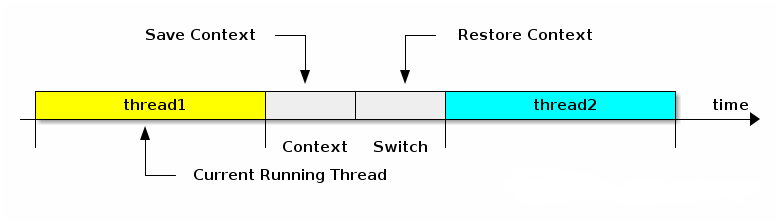
\includegraphics[width=\linewidth]{figures/contextSwitching.png}
	\caption{Promjena konteksta\protect\footnotemark}
	\label{fig:contextSwitching}
\end{figure}

\def\UrlBreaks{\do\/\do-}
\footnotetext{Izvor: \burl{https://developpaper.com/understanding-system-structure-from-java-perspective-1-cpu-context-switch/}}

\section{Kritični odsječak}
Dretve mogu koristiti neke zajedničke resurse. Moguće je istovremeno čitanje zajedničkih resursa, no ako je potrebno promijeniti vrijednost neke varijable moguće je da dvije ili više dretvi to pokušaju učiniti istovremeno. Kako se promjena jedne dretve ne bi izgubila istovremenim pisanjem druge dretve potrebno je osigurati da samo jedna dretva u bilo kojem trenutku može modificirati tu vrijednost. Dio posla koji smije obavljati samo jedna dretva u bilo kojem trenutku naziva se kritični odsječak \engl{critical section}. Kako bi se kritični odsječak zaštitio koriste se sinkronizacijski mehanizmi. U ovom radu korištene su blokirajuće strukture podataka. Kada dretva pokuša koristiti blokirajuću strukturu podataka koju već koristi neka druga dretva ona postaje blokirana, odnosno mora čekati da prva dretva prestane koristiti tu strukturu podataka i tek tada može nastaviti svoje izvođenje \citep{os}.

\chapter{Algoritam računanja histograma orijentacija gradijenata u slikama}
Algoritam računanja histograma orijentacija gradijenata \engl{histogram of oriented gradients} koristi se kako bi se za sliku izračunao njezin opisnik koji sadrži sažete, korisne informacije o toj slici. Dobiveni opisnik može se proslijediti nekom naučenom klasifikatoru koji na temelju njega može odrediti sadrži li slika (ili obrađeni dio slike) traženi objekt. Izračun opisnika se provodi na dijelu slike određene veličine, a točne dimenzije dijela slike koji se koristi ovise o traženom objektu. Glavna ideja je da se traženi objekt može prepoznati pomoću njegovih bridova i orijentacije tih bridova te se zato koristi gradijent.

\section{Izračun gradijenta}
Prije samog izračuna gradijenta moguće je normalizirati boje i gama vrijednosti, ali kako je u originalnom radu \citep{dalal2005histograms} pokazano da to ne utječe značajno na rezultate zbog kasnije normalizacije opisnika, u ovom radu je taj korak preskočen. Za izračun gradijenta sliku je potrebno filtrirati određenom maskom u smjeru \(x\)-osi i \(y\)-osi. U originalnom radu \citep{dalal2005histograms} isprobano je nekoliko tipova maski no najbolja se pokazala jednostavna 1-D centrirana maska koja se zato koristi i u ovom radu: 

\begin{equation}
	[-1, 0, 1]
	\label{eq:mask}
\end{equation}

Uz korištenje maske u formuli \ref{eq:mask} za pojedini piksel \(I\) potrebno je izračunati derivaciju u smjeru \(x\) i \(y\)-osi prema formulama:

\begin{equation}
I_x(r, c) = I(r, c + 1) - I(r, c - 1)
\label{eq:dx}
\end{equation}

\begin{equation}
I_y(r, c) = I(r - 1, c) - I(r + 1, c)
\label{eq:dy}
\end{equation}

U formulama \ref{eq:dx} i \ref{eq:dy} \(r\) predstavlja redak slike, a \(c\) predstavlja stupac slike \citep{tomasi2012histograms}. Ako slika sadrži više boja odnosno kanala, postupak se ponavlja za svaki kanal. Na temelju dobivenih derivacija potrebno je izračunati magnitudu i kut koji će se koristiti u kasnijim koracima:

\begin{equation}
\mu = \sqrt{I_x^2 + I_y^2}
\label{eq:mag}
\end{equation}

\begin{equation}
\theta = \frac{180}{\pi}(\tan_2^{-1}(I_y, I_x) \mod \pi)
\label{eq:ang}
\end{equation}

Kod detekcije pješaka u radu \cite{dalal2005histograms} pokazalo se najbolje koristiti kuteve između 0\degree i 180\degree, odnosno kutevi bez orijentacije, no za neke druge probleme kao što je detekcija automobila pokazalo se bolje koristiti kuteve do 360\degree \citep{dalal2005histograms}. U originalnom radu za doprinos magnitude koristi se magnituda kanala koji ima najveću magnitudu, no u ovom radu koristi se doprinos magnituda svih kanala.

\section{Izračun histograma}
Za izračun histograma prvo treba sliku podijeliti u kvadratne ili kružne ćelije koje se međusobno ne preklapaju. U ovom radu se koriste kvadratne ćelije širine 8 piksela i visine 8 piksela. Slika~\ref{fig:hogCells} prikazuje uvećanu sliku dimenzija 64 na 128 piksela podijeljenu u ćelije dimenzija 8 na 8 piksela.

\begin{figure}[htb]
	\centering
	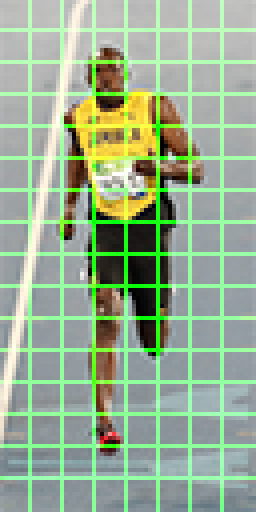
\includegraphics[width=0.3\linewidth]{figures/hog-cells.png}
	\caption{Slika podijeljena u ćelije\protect\footnotemark}
	\label{fig:hogCells}
\end{figure}

\footnotetext{Izvor: \burl{https://www.learnopencv.com/histogram-of-oriented-gradients/}}


Za svaku ćeliju zatim se računa histogram orijentacije gradijenata. U radu \citep{dalal2005histograms} pokazalo se da za detekciju pješaka preciznost rase s povećanjem broja stupaca po histogramu do broja 9 te se zato i u ovom radu koristi upravo devet stupaca. Raspon svakog stupca definiran je formulom:

\begin{equation}
	w = \frac{180}{B}
	\label{eq:width}
\end{equation}

U formuli \ref{eq:width} \(B\) predstavlja broj stupaca \citep{tomasi2012histograms}. Potrebno je izračunati doprinos magnitude za svaki piksel unutar pojedine ćelije. Za izračun doprinosa potrebno je definirati sredinu raspona pojedinog stupca formulom:

\begin{equation}
	c_i = w(i + \frac{1}{2})
	\label{eq:center}
\end{equation}

 U formuli \ref{eq:center} \(w\) predstavlja širinu stupca, a \(i\) indeks stupca. Piksel svojom magnitudom doprinosi stupcu kojem pripada po some kutu i sljedećem stupcu ovisno o udaljenosti kuta od središta stupca kojem pripada, a to je prikazano formulama: 
 
 \begin{equation}
	v_{j} = \mu \frac{c_{j + 1} - \theta}{w}
 	\label{eq:vote}
 \end{equation}
 
 \begin{equation}
 	v_{j+1} = \mu \frac{\theta - c_j}{w}
 	\label{eq:voteNext}
\end{equation}

Zbroj vrijednosti iz formula \ref{eq:vote} i \ref{eq:voteNext} mora biti \(\mu\) jer piksel vrijednosti stupca doprinosi cijelom svojom magnitudom \citep{tomasi2012histograms}. Slika~\ref{fig:vote} prikazuje podjelu doprinosa magnitude \(\mu \) uz kut od 77\degree i devet stupaca po ćeliji. Doprinos stupcu histograma može biti sama vrijednost magnitude, ali može biti i neka druga vrijednost kao kvadrat ili korijen magnitude. U radu \cite{dalal2005histograms} ustanovilo se da se u praksi najbolji rezultati dobiju ako se koristi vrijednost magnitude te je zato ta vrijednost korištena i u ovom radu.

\begin{figure}[htb]
	\centering
	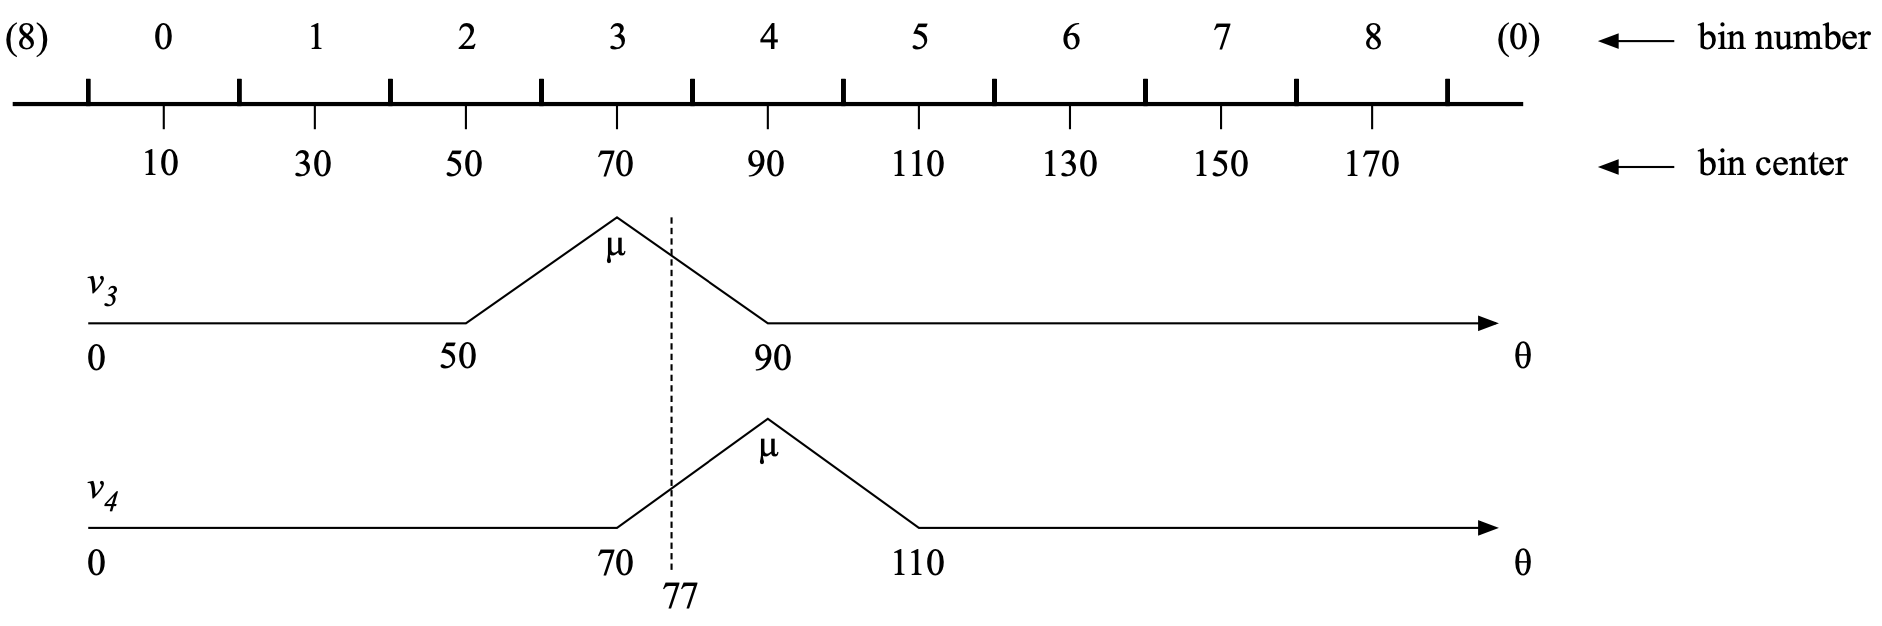
\includegraphics[width=\linewidth]{figures/vote.png}
	\caption{Slika podijeljena u ćelije\protect\footnotemark}
	\label{fig:vote}
\end{figure}

\footnotetext{Izvor: \citep{tomasi2012histograms}}

\section{Normalizacija blokova}
Lokalno osvjetljenje i kontrast mogu znatno utjecati na magnitudu gradijenta. Iz tog razloga vrlo je važno normalizirati blokove susjednih ćelija. Odabrani su blokovi širine 4 i visine 4 ćelije. U radu \cite{dalal2005histograms} ustanovljeno je da preklapanje blokova na pola bloka pozitivno utječe na preciznost detekcije tako da je u ovom radu za pomak bloka korištena jedna ćelija. Vrijednosti u bloku zapisane u obliku vektora normiraju se formulom:

\begin{equation}
	v = \frac{v}{\sqrt{\left\|v\right\|^2 + \epsilon}}
	\label{eq:norm}
\end{equation}

Vrijednost $\epsilon$ u formuli \ref{eq:norm} predstavlja malu pozitivnu konstantu kako bi se izbjeglo potencijalno dijeljenje s nulom \citep{tomasi2012histograms}.

\section{Normalizacija opisnika}
Nakon što su blokovi normalizirani potrebno je sve vrijednosti zapisati kao jedan vektor te taj vektor ponovno normalizirati formulom \ref{eq:norm}. Sada u formuli \ref{eq:norm} \(v\) predstavlja novonastali vektor, a $\epsilon$ ponovno malu pozitivnu konstantu. Još može biti poželjno ograničiti maksimalnu vrijednost $\tau$ kako velike magnitude gradijenta ne bi prikrile detalje. Ovo ograničavanje obavlja se po formuli:

\begin{equation}
	v_n = \min(v_n, \tau)
	\label{eq:limit}
\end{equation}

Nakon toga dobiven vektor još se jednom normalizira. Tako izračunati vektor predstavlja opisnik slike. Ovime je slika dimenzija 64 na 128 piksela sažeta na opisnik koji sadrži 15 horizontalnih i 7 vertikalnih blokova koji svaki sadrži po 4 ćelije odnosno histograma s 9 stupaca. Dakle slika koja ukupno ima 8196 piksela od kojih svaki može sadržavati informacije o četiri kanala sažeta je u jedan opisnik kosi ima samo 3780 vrijednosti neovisno o broju kanala \citep{tomasi2012histograms}. Takvi opisnici mogu se koristiti kako bi se naučili modeli za klasifikaciju te kasnije i za samu klasifikaciju odnosno detekciju ima li slika traženi objekt.

\chapter{Detekcija pješaka}
Kako bi izračunati opisnici mogli biti korisni potrebno je odabrati klasifikator koji će biti treniran na skupu opisnika izračunatih za zadani skup slika za treniranje. U originalnom radu \cite{dalal2005histograms} kao klasifikator koristi se stroj potpornih vektora te je zato isti korišten u ovom radu.

\section{Stroj potpornih vektora}
Stroj potpornih vektora \engl{Support Vector Machine, SVM} je klasifikator koji razrede odvaja izračunom optimalne hiperravnine u fazi učenja. Za učenje se koristi tehnika nadzirano učenje što znači da se modelu predaju primjeri izračunatih opisnika i labela predstavlja li taj opisnik sliku koja sadrži traženi objekt ili ne \citep{svm}. Opisani klasifikator je linearni klasifikator i daje samo pozitivne ili negativne odgovore. Slika~\ref{fig:hyperplane} prikazuje dobivenu optimalnu hiperravninu za linearni klasifikator.

\begin{figure}[htb]
	\centering
	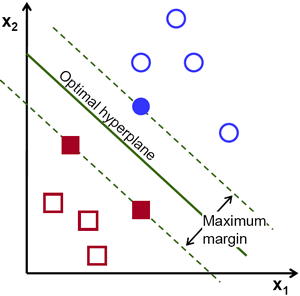
\includegraphics[width=0.5\linewidth]{figures/optimal-hyperplane.png}
	\caption{Prikaz hiperravnine\protect\footnotemark}
	\label{fig:hyperplane}
\end{figure}

\footnotetext{Izvor: \burl{https://docs.opencv.org/3.4/d1/d73/tutorial_introduction_to_svm.html}}

U originalnom radu \cite{dalal2005histograms} korišten je skup podataka INRIA\protect\footnotemark, ali u vrijeme pisanja ovog rada web stranica nije bila dostupna tako da je korišten skup podataka koji su prikupili kolege u prijašnjim godinama.

\footnotetext{Izvor: http://pascal.inrialpes.fr/data/human/}

\section{Klizni prozor}
Slika na temelju koje se može izračunati ima unaprijed određene dimenzije. No često će se dogoditi da treba analizirati sliku koja je većih dimenzija. Tada je potrebno iskoristiti koncept kliznog prozora. Klizni prozor je prozor dimenzija slike pomoću koje algoritam može izračunati opisnik (dakle u ovom slučaju visine 128 i širine 64 piksela) koji se pomiče po slici koja se trenutno analizira. Na svakoj poziciji ne koju prozor dođe potrebno je izračunati opisnik i predati ga klasifikatoru. Kako bi računanje opisnika za svaku moguću poziciju dugo trajalo i ne bi znatno poboljšalo rezultate obično se definira korak za koliko piksela se prozor pomiče u svakoj iteraciji.

\section{Piramida slike}
Koncept kliznog prozora riješio je problem analize većih slika, no i dalje postoji mogućnost da je traženi objekt na trenutnoj slici veći od definiranih dimenzija dijela slike na temelju kojega se izračunava opisnik. Kada se koristi piramida slike prvo se analizira originalna slika, a zatim se ta slika smanjuje za neki definirani faktor te se na smanjenoj slici ponovno provodi analiza tehnikom kliznog prozora i izračunom opisnika za svaku poziciju. Postupak smanjivanja i analize smanjene slike se ponavlja dok smanjivanje slike ne bi rezultiralo slikom čija je jedna ili obije stranice manja od dimenzija prozora na temelju kojeg se izračunava opisnik.

\chapter{Programsko rješenje}
Za implementaciju ovog rada odabran je programski jezik Java. Za lakšu organizaciju projekta i potrebnih biblioteka, kao i za automatizaciju prevođenja i povezivanja potrebnih biblioteka koriśten je alat Apache Maven. Radi jednostavnijeg i efikasnijeg ostvarenja operacija koje nisu tema ovog rada koristi se biblioteka OpenCV. \\

Radi lakšeg korištenja i lakše vizualizacije raznih operacije koje se koriste u izračunu opisnika program je ostvaren kao jednostavna grafička aplikacija. Većina opcija ostvarena je kroz gumbe koji se nalaze pri dnu grafičkog sučelja. Ako neku opciju trenutno nije moguće izvesti jer nema učitane slike pritisak gumbe bit će ignoriran, a ako je odabranu opciju moguće izvest, ali je došlo do pogreške korisnik će biti obaviješten. Slika~\ref{fig:initialGui} prikazuje grafičko sučelje i originalne postavke po pokretanju programa.

\begin{figure}[htb]
	\centering
	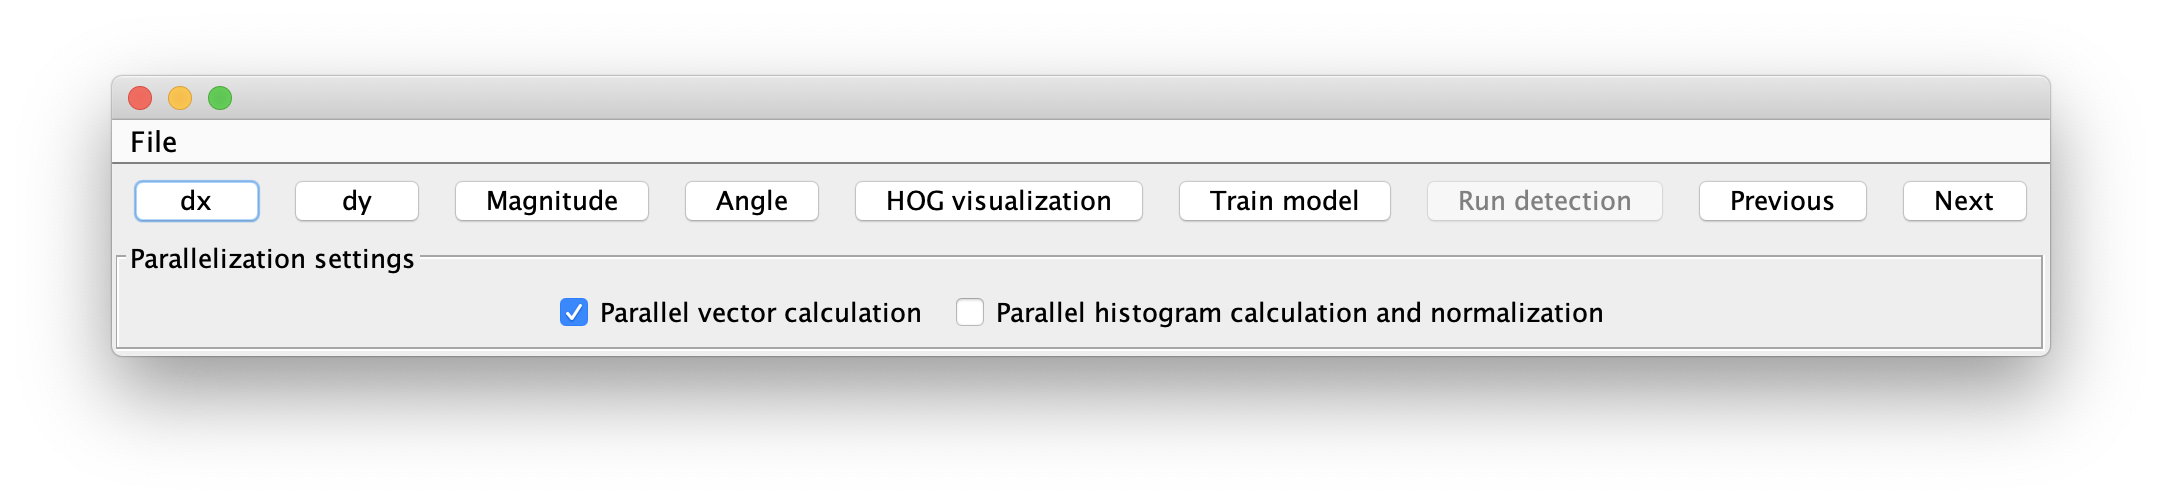
\includegraphics[width=\linewidth]{figures/initialGui.png}
	\caption{Grafičko sučelje nakon pokretanja}
	\label{fig:initialGui}
\end{figure}

\section{Učitavanje slike}
Kako bi se mogao izračunati opisnik neke slike ili pokrenuti detekcija objekata na slici potrebno je sliku prvo učitati. Odabirom izbornika \textit{File} pa \textit{Open} otvara se prozor u kojem je moguće izabrati sliku koja će se koristiti. Slika se zatim čuva kao objekt Javinog razreda \verb|BufferedImage| kako bi se mogla prikazati ne grafičkom sučelju i kako bi se mogli koristiti podaci iz slike. Razred \verb|Algorithms| sadrži brojne statičke metode kojima se može pristupiti podacima slike kao i metode potrebne za izračun gradijenta. Učitana slika se pretvara u niz tipa \verb|float| korištenjem metode \verb|getDataFloat()|. Sliku je moguće učitati i kao niz tipa \verb|int| metodom \verb|getDataInt()| gdje svaki broj predstavlja jedan piksel. Kako je programski lakše koristiti prikaz tipa \verb|float| gdje svaka vrijednost predstavlja vrijednost jednog kanala piksela u rasponu od 0 do 1, u nastavku rada koristi se taj prikaz. Reprezentacija slike mogla je biti riješena korištenjem trodimenzionalnog polja gdje dimenzije predstavljaju širinu, visinu i kanale slike ili korištenjem razreda \verb|Mat| biblioteke OpenCV, ali izabrano je jednodimenzionalno polje jer je to najjednostavniji prihvatljivi tip objekta. Slika~\ref{fig:loadedImage} prikazuje grafičko sučelje s učitanom slikom iz skupa za učenje.

\begin{figure}[htb]
	\centering
	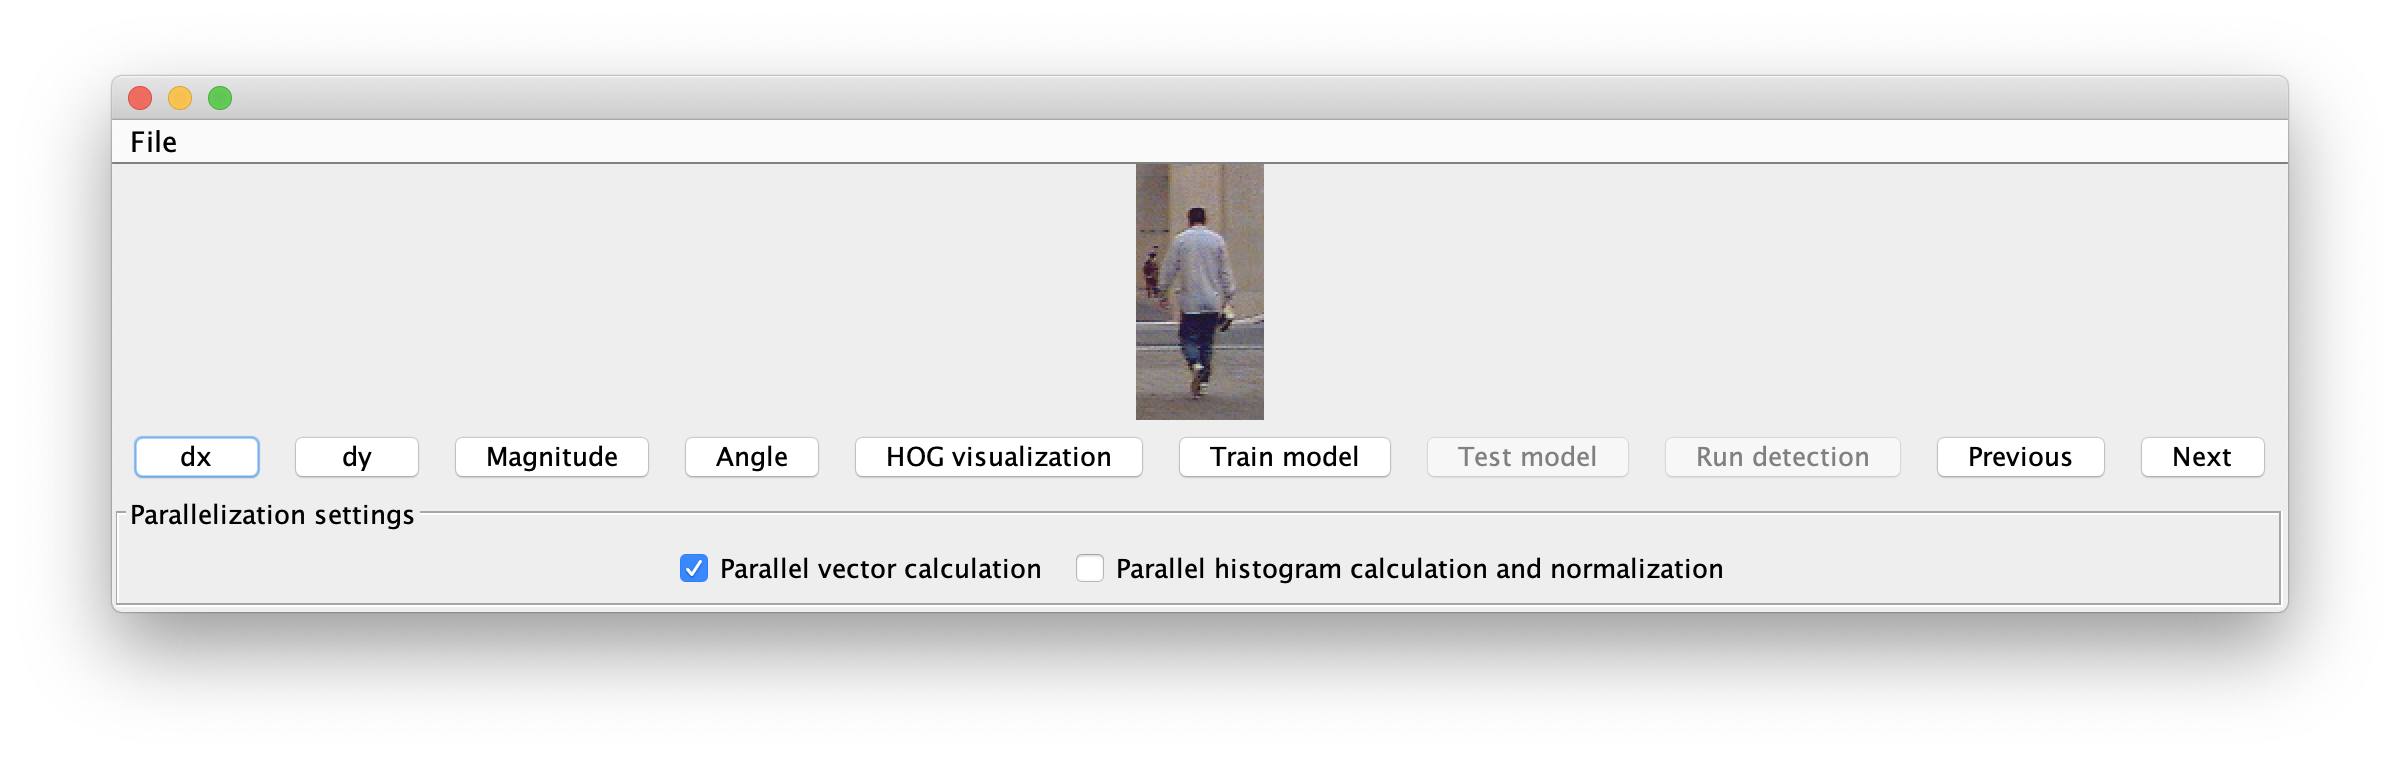
\includegraphics[width=\linewidth]{figures/loadedImage.png}
	\caption{Prikaz učitane slike}
	\label{fig:loadedImage}
\end{figure}

\section{Računanje gradijenta}
Nakon što je slika uspješno učitana pojedinačno ili kao primjer u skupu za učenje potrebno je izračunati gradijente u smjeru \(x\) i \(y\)-osi. U ovom koraku postoji opcija paralelizacije. Za izračun se koristi funkcija \verb|derive()| koja prima sliku kao polje tipa \verb|float|, znak 'x' ili 'y' koji određuje smjer derivacije, podatke o širini, visini i broju kanala te konačno zastavicu tipa \verb|bool| koja određuje izvodi li se izračun paralelizirano ili ne. Za paralelizaciju se koristi Javin razred \verb|Thread|. Iz blokirajućeg reda \verb|BlockingQueue| dretve izvlače indekse koji predstavljaju stupac ili redak slike za koji treba izračunati derivaciju. Dretve rade u beskonačnoj petlji dok ne izvuku \verb|killElement| koji im signalizira prekid rada, a takvi elementi nalaze se na kraju reda i ima ih koliko i pokrenutih dretvi. Svaka metoda koja koristi paralelizaciju prvo traži broj dostupnih procesorskih jezgri metodom \verb|availableProcessors()| razreda \verb|Runtime| i pokreće upravo toliko dretvi kako ne bi došlo do nepotrebnih promjena konteksta. Nakon što su dretve pokrenute poziva se statička metoda \verb|joinThreads()| razreda \verb|Algorithms| kojoj se predaje polje pokrenutih dretvi kako bi glavna dretva bila blokirana dok sve dretve ne završe svoj posao, čime se postiže maksimalna efikasnost. \\

Pritiskom na gumbe \textit{dx} ili \textit{dy} grafičkog sučelja pokreće se paralelizirani izračun odabrane derivacije učitane slike. Nakon što je derivacija izračunata umjesto slike na sučelju se prikazuje vizualizacija dobivene derivacije generirana statičnom metodom \verb|convertToImage()| razreda \verb|Algorithms| koja iz polja tipa \verb|float| napravi sliku tipa \verb|BufferedImage|. Slika~\ref{fig:dx} pokazuje derivaciju u smjeru \(x\)-osi dok slika~\ref{fig:dy} pokazuje derivaciju u smjeru \(y\)-osi. Prikazana slika je iz skupa za testiranje. Za prikaz he izabrana slika većih dimenzija kako bi se bolje vidjeli detalji i kako bi se pokazalo da ove metode rade neovisno o dimenzijama slike.

\begin{figure}[htb]
	\centering
	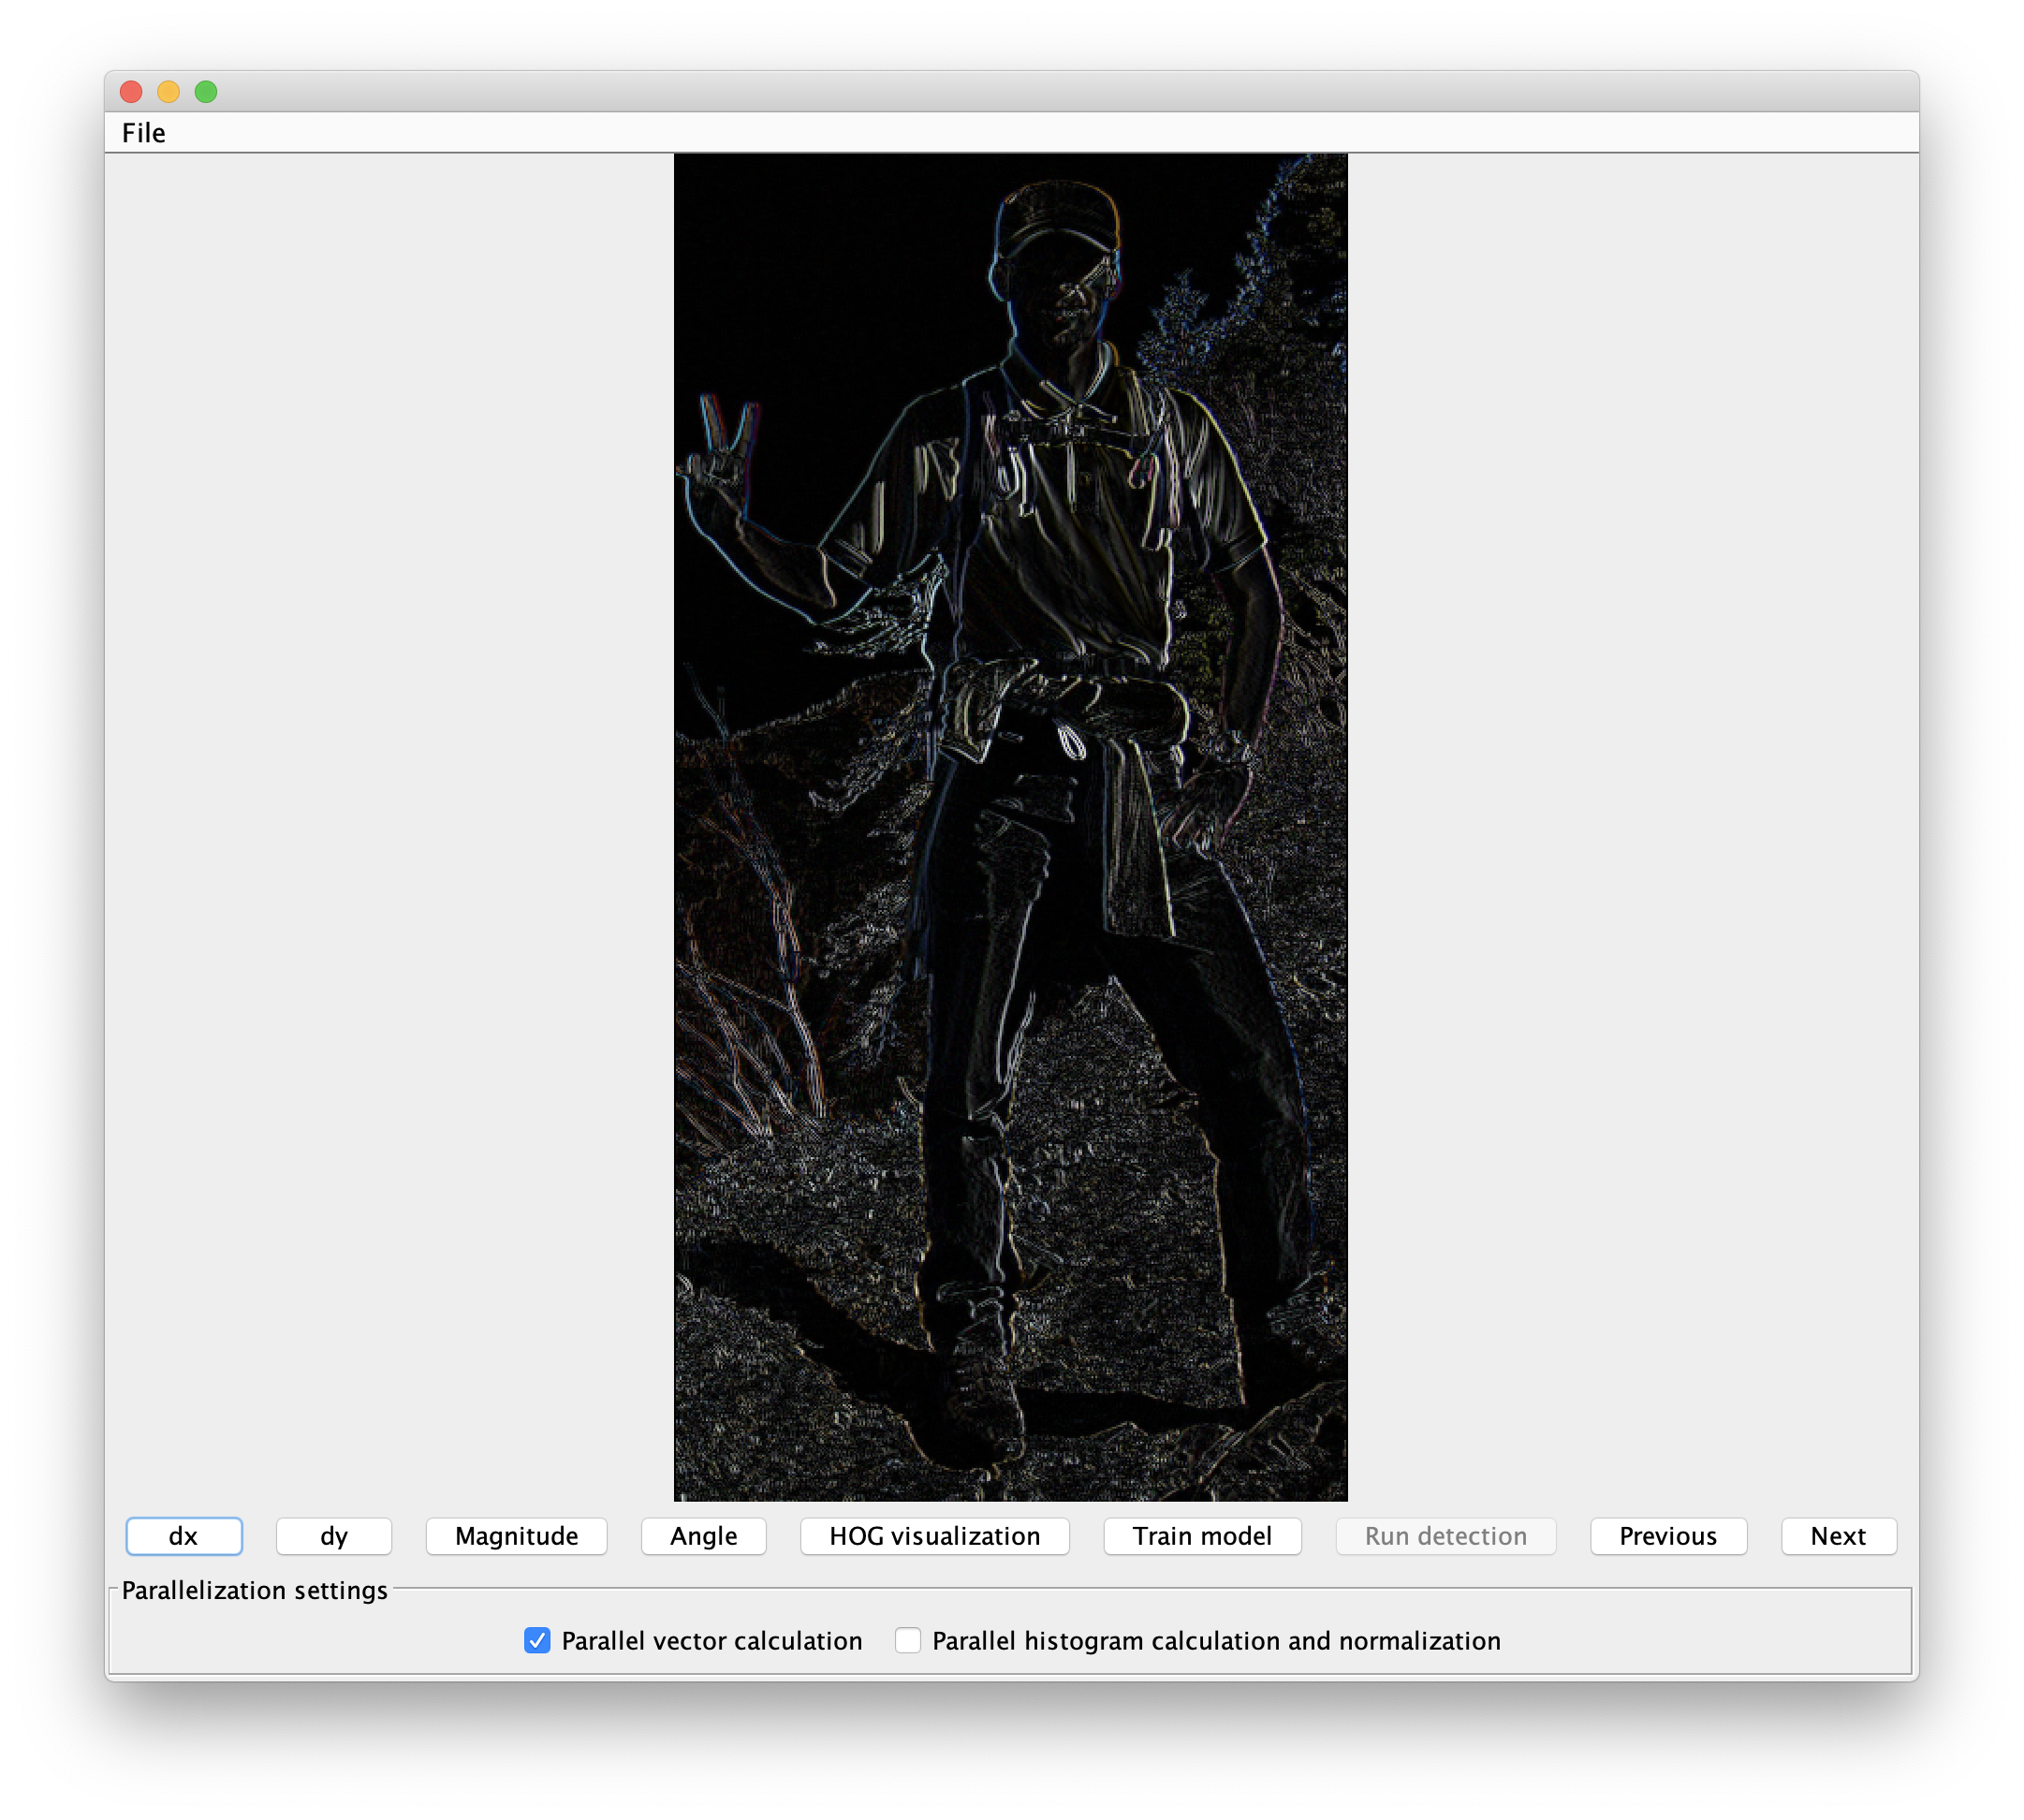
\includegraphics[width=0.75\linewidth]{figures/dx.png}
	\caption{Derivacija u smjeru \(x\)-osi}
	\label{fig:dx}
\end{figure}

\begin{figure}[htb]
	\centering
	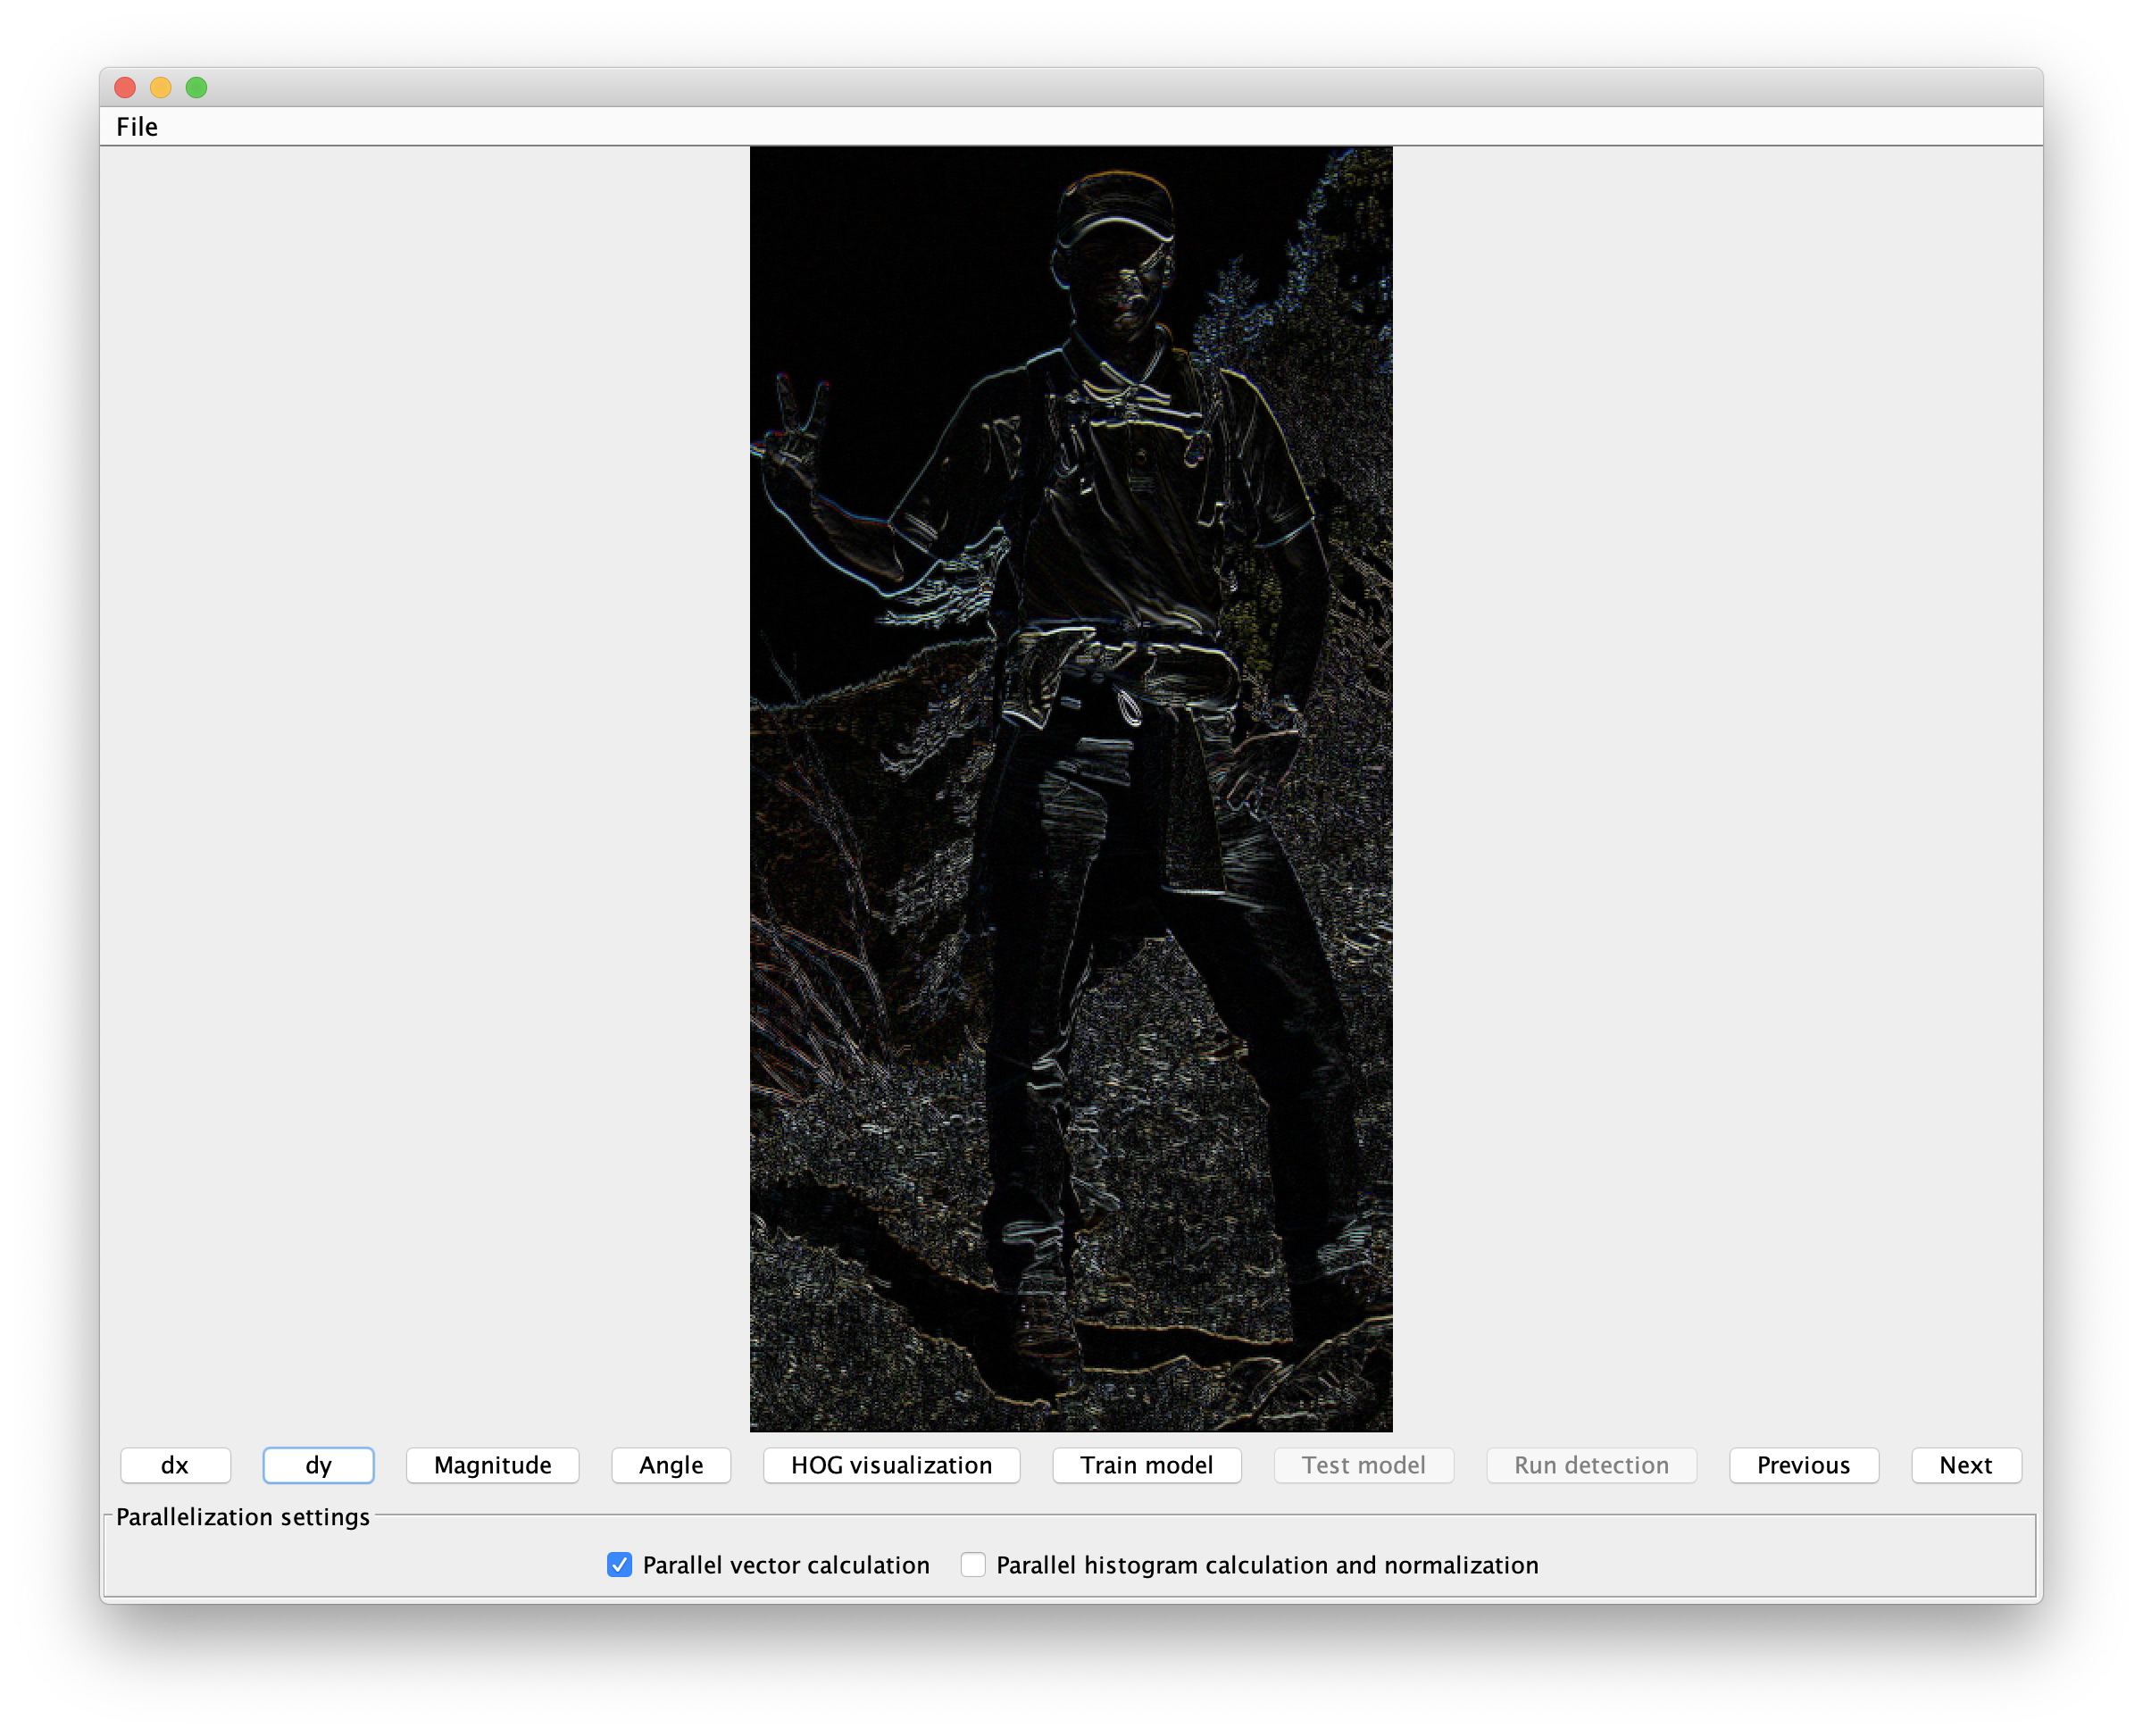
\includegraphics[width=0.75\linewidth]{figures/dy.png}
	\caption{Derivacija u smjeru \(y\)-osi}
	\label{fig:dy}
\end{figure}

\section{Izračun magnitude i kuta}
Magnituda je izračunate po formuli \ref{eq:mag}, a kut po formuli \ref{eq:ang}. Kako su oboje relativno jednostavne operacije i ne ovise o pojedinom retku ili stupcu ovdje nije korištena nikakva paralelizacija. Vizualizacija je ponovno ostvarena metodom \verb|convertToImage()|. Pritiskom na gumb \textit{Magnitude} prikazuje se vizualizacija magnitude, a pritiskom na gumb \textit{Angle} prikazuje se vizualizacija kuta. Iako se na vizualizaciji kuta ne vidi ništa što  ljudskom oku izgleda smisleno, ona je ostavljena radi kompletnosti. Slika~\ref{fig:magnitude} prikazuje vizualizaciju magnitude slike korištene u slikama \ref{fig:dx} i \ref{fig:dy}.

\begin{figure}[htb]
	\centering
	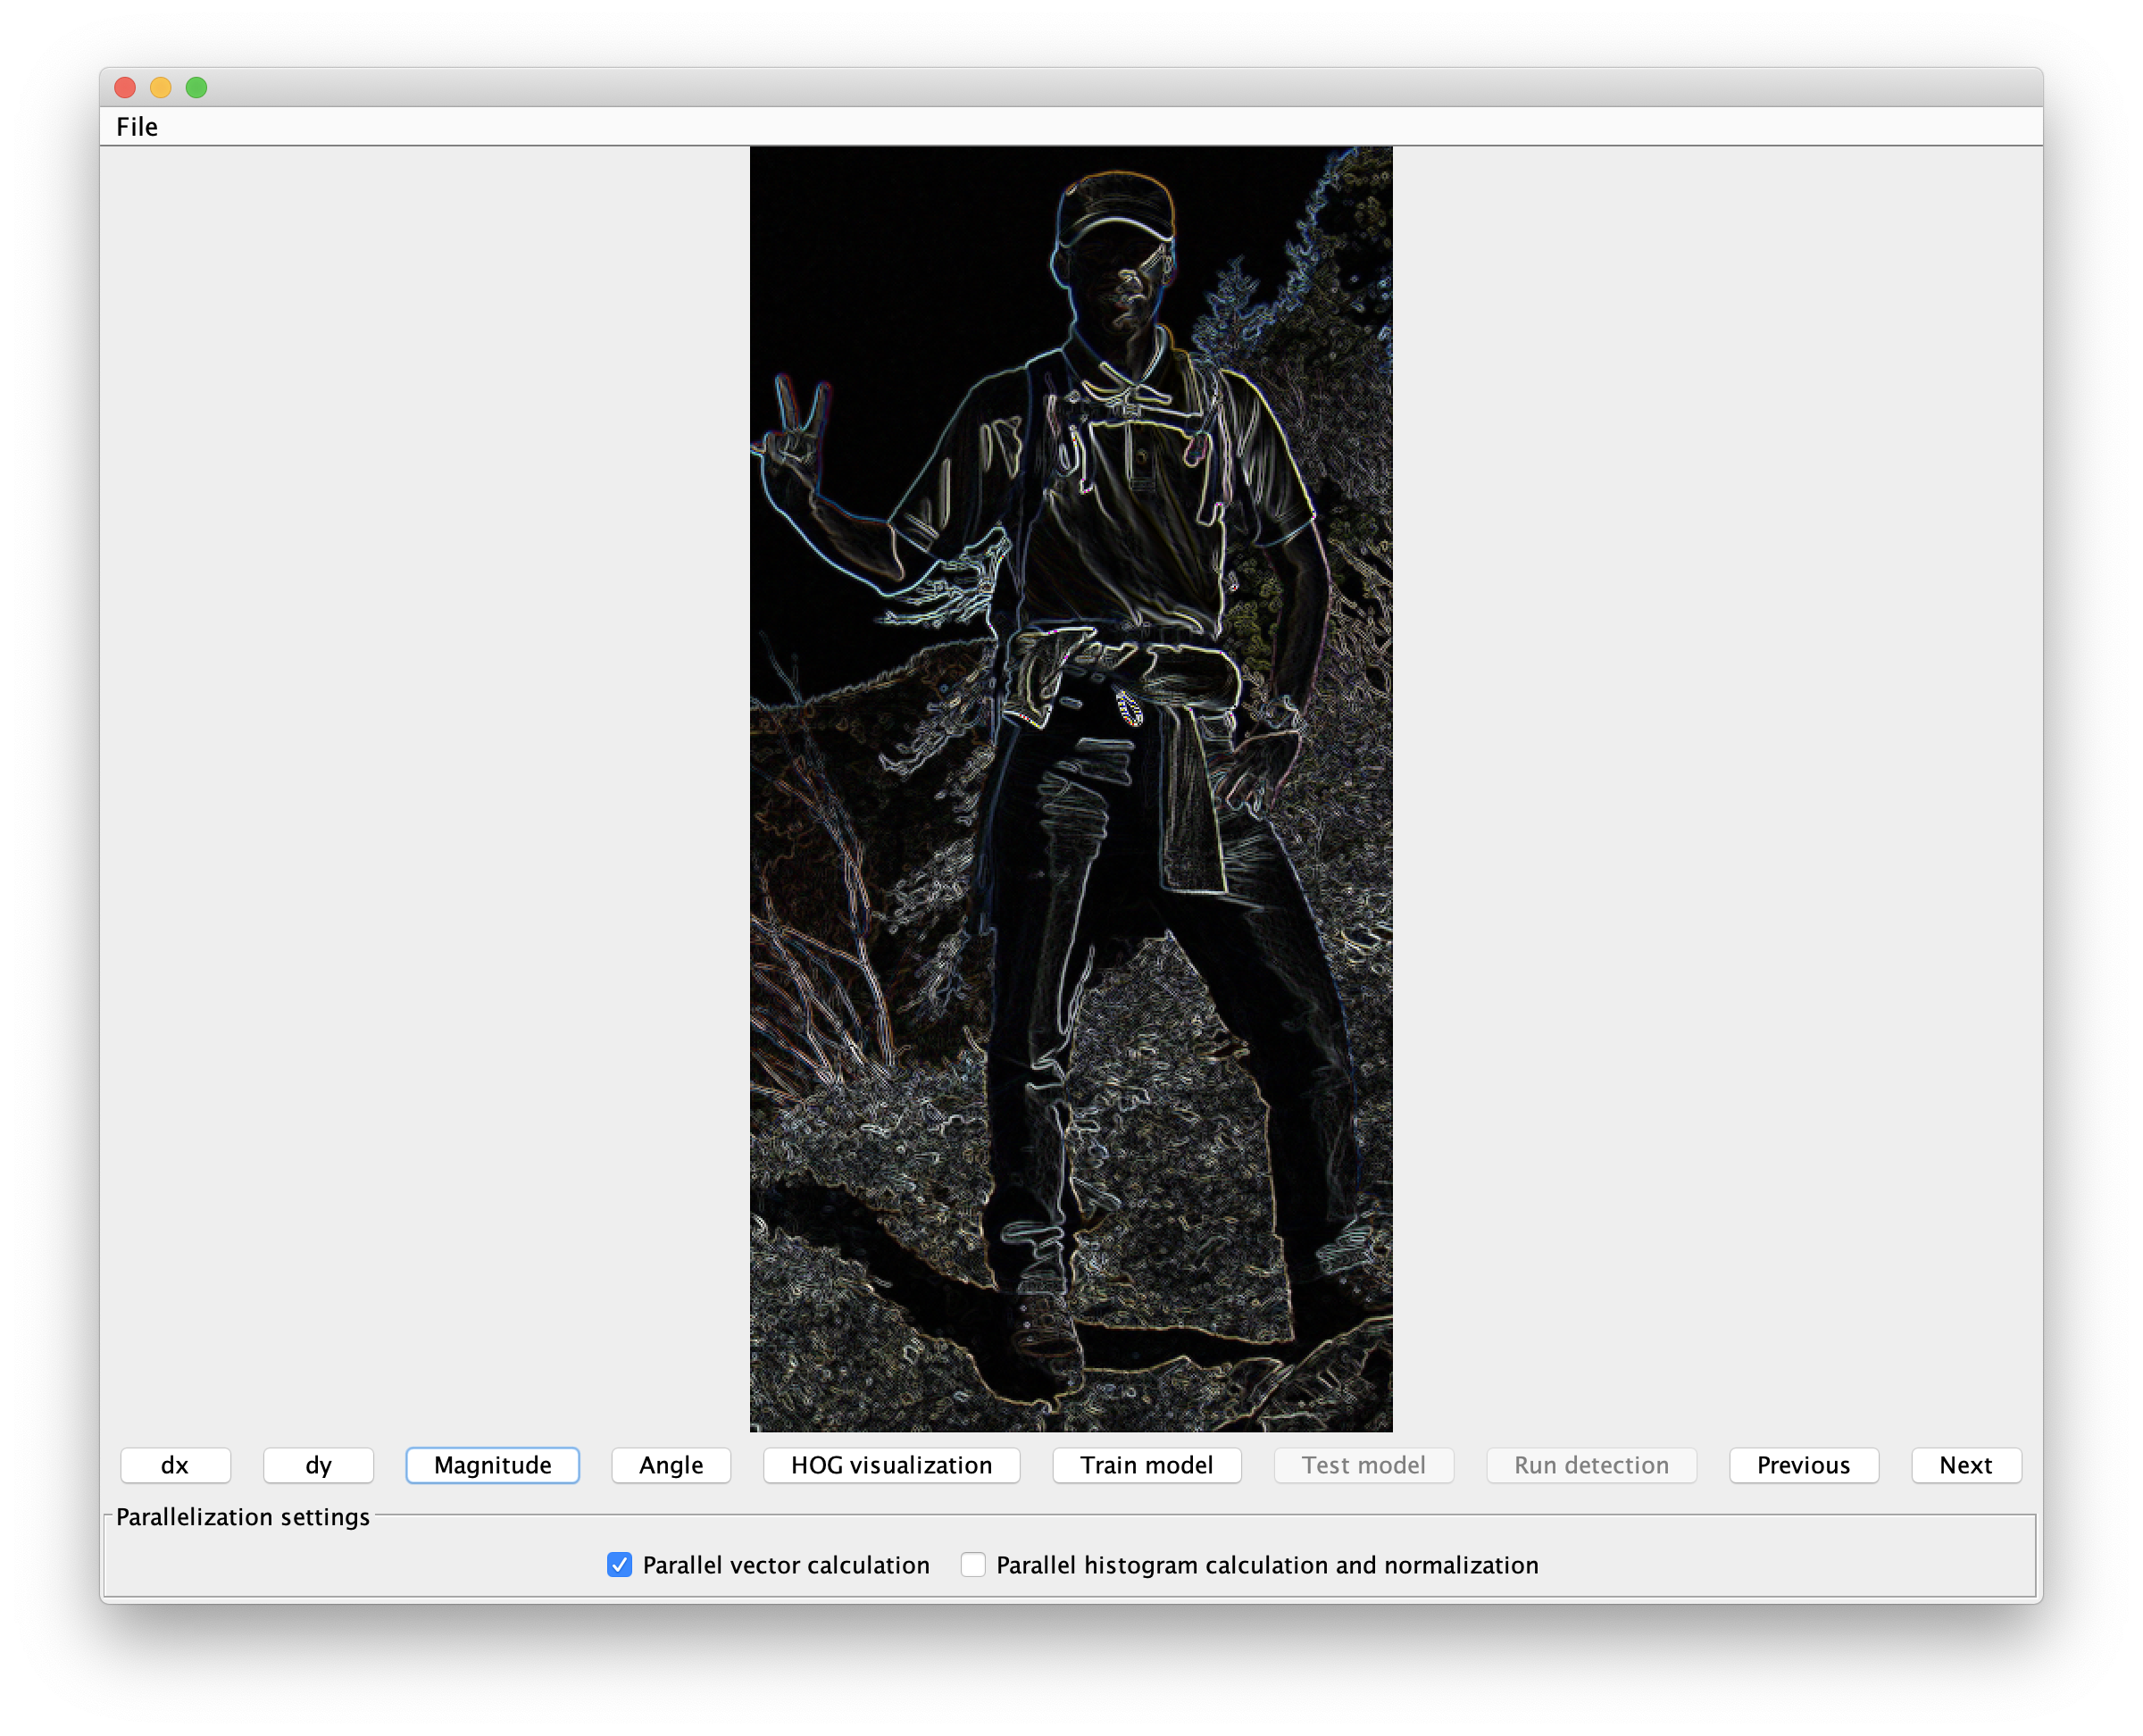
\includegraphics[width=0.75\linewidth]{figures/magnitude.png}
	\caption{Vizualizacija magnitude}
	\label{fig:magnitude}
\end{figure}

\section{Izračun histograma}
Za daljnju obradu slika koristi se razred \verb|HOGImage|. Razred ima dva konstruktora. U jednom prima objekt tipa \verb|BufferedImage| pomoću kojeg sam doznaje korisne informacije o slici i računa gradijent po prethodno opisanom postupku. Drugi konstruktor prima već izračunatu magnitudu i kut te informacije o dimenzijama originalne slike. Razred definira dva očekivana načina korištenja ovisno o tome je li slika predviđenih dimenzija ili je potrebno koristiti klizni prozor. Ovdje je detaljnije objašnjen način rada kada se koristi slika predviđenih dimenzija. Kod korištenja kliznog prozora koristi se ista funkcionalnost koja je ovdje objašnjena, ali uz drugačije opcije paralelizacije radi veće efikasnosti. Vrijednosti histograma se računaju pozivom metode \verb|calculateHistogram()|. Metoda ne prima nikakve argumente već je sama po sebi paralelizirana. Slika dužine 64 i visine 128 piksela se podijeli u kvadratne ćelije dimenzije 8 piksela. Svaka ćelija predstavlja histogram s 9 stupaca, a svaki stupac pokriva širinu od 20\degree. U blokirajući red se stavljaju indeksi na temelju kojih se računa odmak do početnog elementa ćelije koju taj indeks predstavlja. Zatim se dretvama predaje taj red te se one pokreću, a glavna dretva se blokira dok ostale ne završe s radom. Dretve prestaju s radom kada dobiju index \verb|-1|. Kako svaka dretva upisuje izračunati histogram u polje na lokaciju izvučenog indeksa, a zbog korištenja blokirajućeg reda nije moguće da dvije dretve izvuku isti indeks, kod zapisivanja histograma nije potrebno koristiti sinkronizacijski mehanizam. U dretvama se doprinos magnitude računa prema formulama \ref{eq:vote} i \ref{eq:voteNext}.

\section{Normalizacija blokova}
Nakon izračunatih histograma potrebno je normalizirati blokove po formuli \ref{eq:norm}. Za slike širine 64 i visine 128 piksela to se računa metodom \verb|normalizeBlocks()|. Kao i kod računanja histograma metoda ne prima nikakve parametre, već se samo izvodi paralelno. Na sličan način blokovi su reprezentirani indeksima pomoću kojih si izračunava početni histogram bloka. Blokovi se normaliziraju paralelno te se rezultati zapisuju u novo polje. Kako se histogrami samo čitaju, a u polje s normaliziranim blokovima svaka dretva upisuje rezultat na svoj indeks, za te operacije nije potrebno ostvariti mehanizme sinkronizacije. Za parametar $\epsilon$ odabrana je vrijednost \(10^{-5}\).

\section{Normalizacija opisnika}
Zadnji korak u izračunu opisnika je normalizacija normaliziranih blokova zapisanih kao jedan vektor, ograničavanje maksimalne vrijednosti prema formuli \ref{eq:limit} te ponovna normalizacija dobivenog vektora. Kako je ovo relativno jednostavna operacija i za normalizaciju je potrebno sumirati sve vrijednosti vektora što bi kod paralelizacije predstavljalo kritični odsječak, ova operacija nije paralelizirana. Vrijednost parametra $\tau$ postavljena je na \(0.2\) kao i radu \cite{tomasi2012histograms}.

\section{Vizualizacija rezultata}
Ako je učitana slika širine 64 i visine 128 piksela pritiskom na gumb \textit{HOG visualization} preko slike se iscrtavaju normalizirane vrijednosti histograma. U svakoj ćeliji iscrtane su crte duljine proporcionalne vrijednostima svog stupca histograma i zarotiran za kut koji predstavlja centar stupca. U takvoj vizualizaciji najdulje linije bit će okomite na prepoznate rubove. Vizualizacija pomaže da bi korisnik shvatio kako računalo "vidi" sliku. Za iscrtavanje slike koristi se razred \verb|HOGIcon| koji nasljeđuje Javin razred \verb|ImageIcon|. U konstruktoru prima polje koje sadrži vrijednosti histograma i pomoću afinih transformacija iscrtava linije okrenute za odgovarajući kut. Slika~\ref{fig:hog} prikazuje vizualizaciju histograma na slici iz seta za učenje.

\begin{figure}[htb]
	\centering
	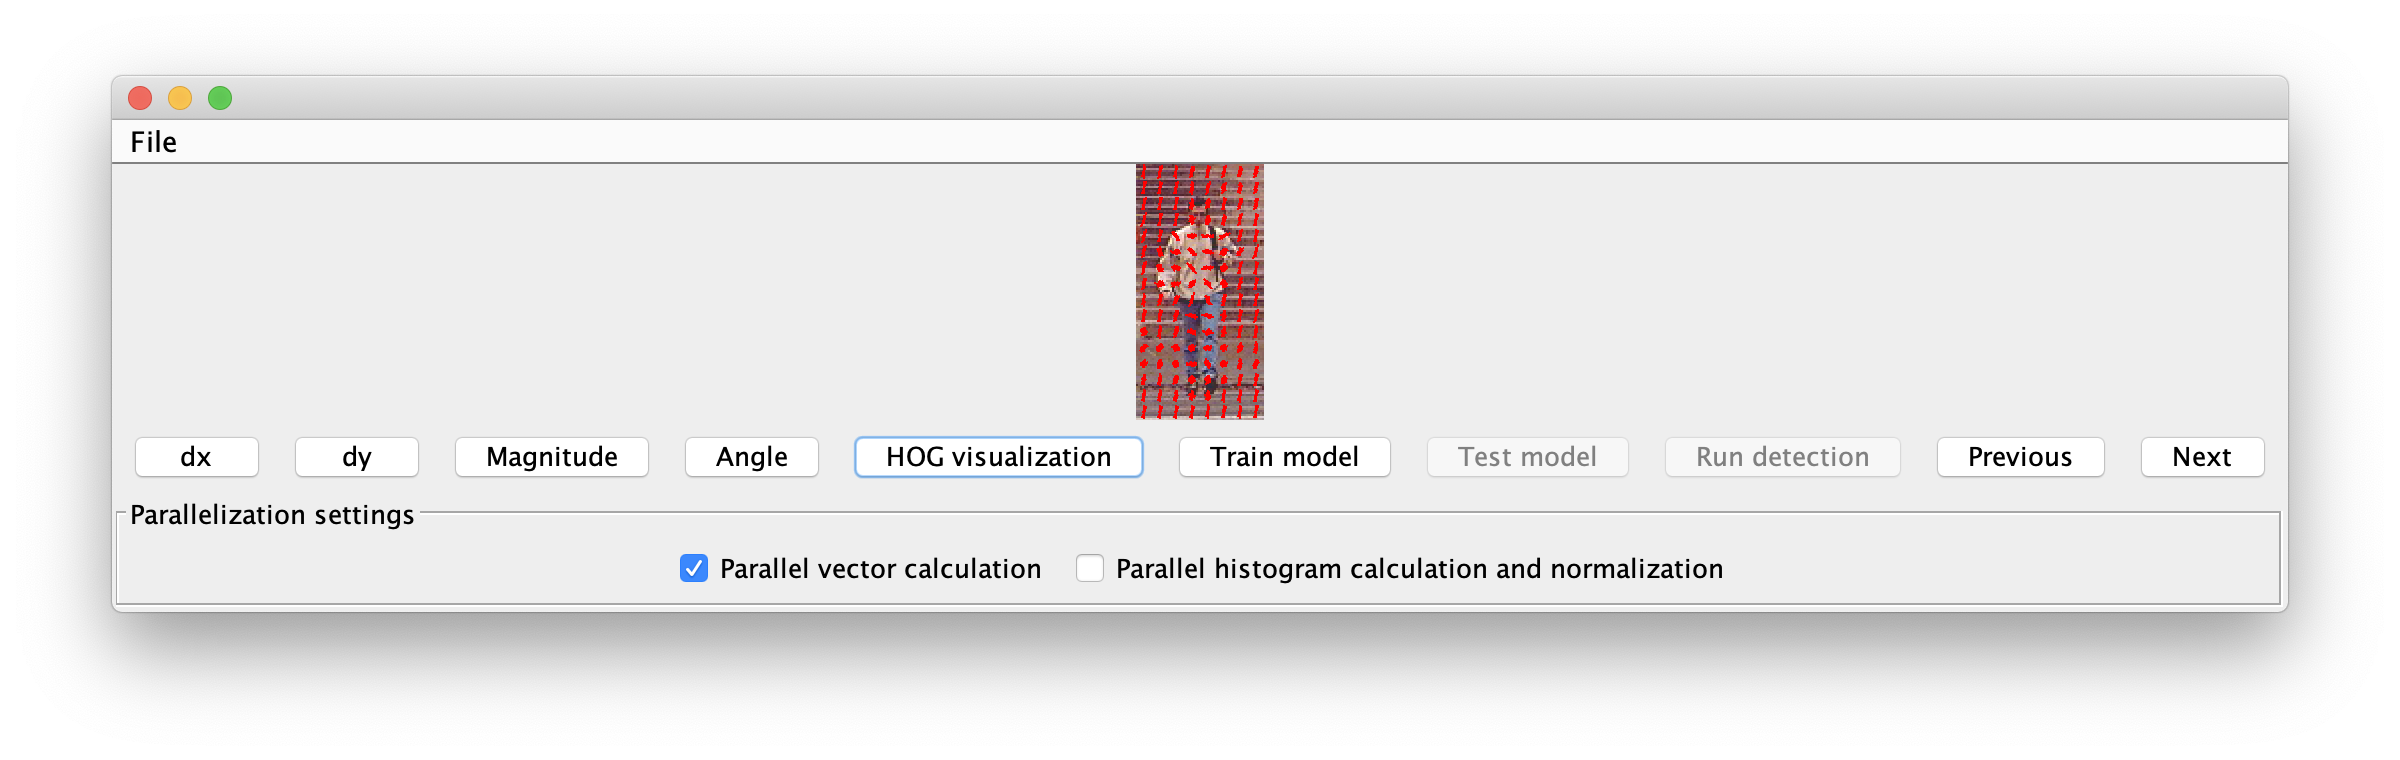
\includegraphics[width=\linewidth]{figures/hogVisualization.png}
	\caption{Vizualizacija histograma po čelijama}
	\label{fig:hog}
\end{figure}

\section{Klizni prozor}
Kako bi se mogla provesti detekcija na slikama većih dimenzija od 64 piksela širine i 128 piksela visine potrebno je ostvariti klizni prozor i piramidu slike. Klizni prozor je istih dimenzija kao i prozor za izračun opisnika, a za pomak prozora koristi se korak od 5 piksela. Proces pomicanja kliznog prozora i izračuna opisnika za svaku poziciju pokreće se metodom \verb|slideWindow()| razreda \verb|HOGImage|. Metoda ima dvije opcije za paralelizaciju koje se mogu mijenjati postavkama na grafičkom sučelju. Prva zastavica za paralelizaciju \verb|parallel| kontrolira hoće li se opisnici za svaku poziciju prozora računati paralelno ili ne. Pozicija prozora se ponovno računa pomoću indeksa. Polja koja sadrže magnitudu i kut slike izračunata su za cijelu sliku pri konstrukciji objekta \verb|HOGImage| i koriste se samo za čitanje tako da u slučaju paralelnog izračuna više pozicija prozora nije potrebno koristiti mehanizme sinkronizacije ili prepisivati vrijednosti u novo polje. \\

Druga zastavica za paralelizaciju \verb|parallelChildren| pokreće paralelni izračun histograma i normalizacije blokova unutar pojedinog prozora kako je objašnjeno u ranijim poglavljima. Moguće je koristiti proizvoljnu kombinaciju ovih opcija, ali to može dovesti do velikog broja dretvi koje pokušavaju raditi istovremeno što dovodi do čestih promjena konteksta. Rezultat izvođenja ove metode je polje koje sadrži niz izračunatih opisnika za sve pozicije kliznog prozora na učitanoj slici.

\section{Piramida slike}
Zadnji korak potreban za potpunu analizu slika većih dimenzija je izrada piramide slike i analiza svih njezinih razina. Za smanjenje slika koristi se biblioteka OpenCV. Za faktor skaliranja odabrana je vrijednost \(1.5\). Slike se učitaju kao objekti razreda \verb|Mat| te se skaliraju statičkom metodom \verb|resize()| razreda \verb|Imgproc| biblioteke OpenCV. Piramida slike predstavljena je listom objekata tipa \verb|HOGImage|, a tu listu stvara statička metoda \verb|createPyramid()|. Slike se skaliraju zadanim faktorom sve dok skaliranje ne bi rezultiralo slikom čija je jedna stranica manja od minimalnih dimenzija prozora za detekciju i izračun opisnika. Nakon što je slika skalirana stvara se objekt razreda \verb|HOGImage|, a izračun gradijenta je paraleliziran.

\section{Klasifikator za detekciju objekata}
Potrebno je provjeriti točnost implementiranog postupka, a najbolji način za to je ostvariti jednostavnu implementaciju klasifikatora. Kako implementacija klasifikatora nije tema ovog rada, za klasifikator je odabran razred \verb|SVM| biblioteke OpenCV. Korišten je linearni klasifikator koje određuje je li pronađen pješak ili ne. Na ulaz klasifikatora dovode se izračunati opisnici, a izlaz je pozitivna ili negativna klasifikacija.

\section{Učenje modela}
Da bi se klasifikator mogao koristiti za detekciju, prvo je potrebno trenirati klasifikator na skupu podataka s označenim labelama. Proces treniranja klasifikatora pokreće se pritiskom na gumb \textit{Train model} na grafičkom sučelju. Potrebno je odabrati direktorij koji sadrži direktorije \textit{pos} i \textit{neg}. Direktorij \textit{pos} sadrži slike koji predstavljaju pozitivne primjere i očekivani omjer dimenzija slika je \(1 : 2\). Ako neku sliku nije moguće skalirati na širinu 64 i visinu 128 piksela, taj primjer se odbacuje. Direktorij \textit{neg} sadrži negativne primjere koji mogu biti proizvoljnih dimenzija. Za svaki negativni primjer slučajno se bira \(10\) indeksa na temelju kojih se izračunavaju opisnici. Po učitavanju slike se spremaju u blokirajući red. Pokreću se dretve koje iz tog reda uzimaju slike i na temelju njih računaju opisnike. Izračunati opisnici spremaju se u drugi blokirajući red. Nakon što dretve završe posao glavna dretva sprema sve opisnike iz blokirajućeg reda za pojedini podskup u polje. Stvara se polje koje veličinom odgovara ukupnom broju pozitivnih i negativnih primjera i puni se labelama. Opisnici iz ona polja zapisuju se kao objekt tipa \verb|Mat| i zajedno s poljem labela predaju klasifikatoru kao skup za treniranje. Nakon što je treniranje uspješno završeno moguće je koristiti gumb \textit{Run detection}.  Obavijest o napretku nije vidljiva na korisničkom sučelju jer je za ažuriranje obično zadužena posebna dretva što bi u ovom slučaju narušilo efikasnost procesa učenja.

\section{Detekcija objekta}
Nakon šo je klasifikator uspješno naučen i slika je učitana u grafičko sučelje moguće je pokrenuti detekciju na toj slici pritiskom na gumb \textit{Run detection}. Postavke za paralelizaciju detekcije moguće je definirati na samom korisničkom sučelju. Nakon što je detekcija završila za sve razine piramide na korisničko sučelje postavlja se ikona tipa \verb|DetectionIcon| na kojoj su zelenom bojom označeni pravokutnici koji predstavljaju prozor u kojem je detektiran pješak. Pritiskom na gumbe \textit{Next} i \textit{Previous} moguće je mijenjati prikazanu razinu piramide slike i tako vidjeti rezultate detekcije za  ostale razine. Slika~\ref{fig:detection} prikazuje detekciju pješaka na originalnoj slici, a slika~\ref{fig:scaledDetection} prikazuje uspješnu detekciju tek na zadnjoj razini piramide.

\begin{figure}[htb]
	\centering
	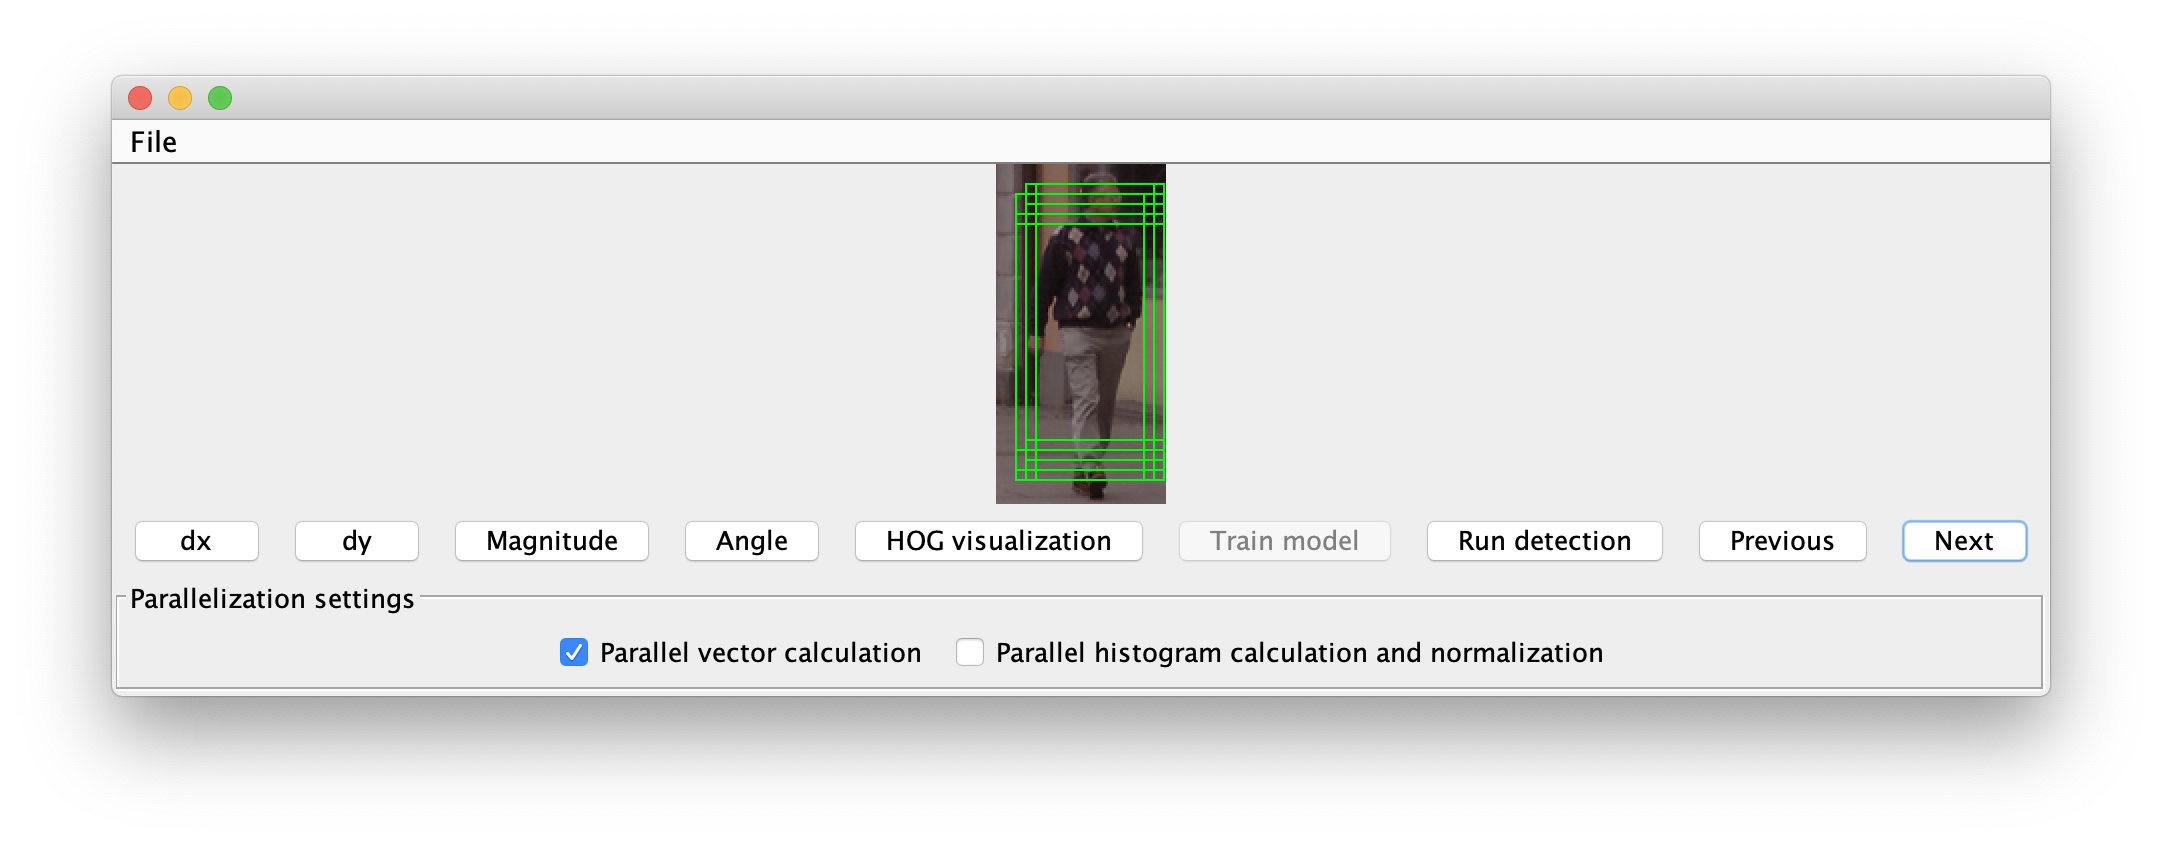
\includegraphics[width=\linewidth]{figures/detection.png}
	\caption{Detekcija pješaka}
	\label{fig:detection}
\end{figure}

\begin{figure}[htb]
	\centering
	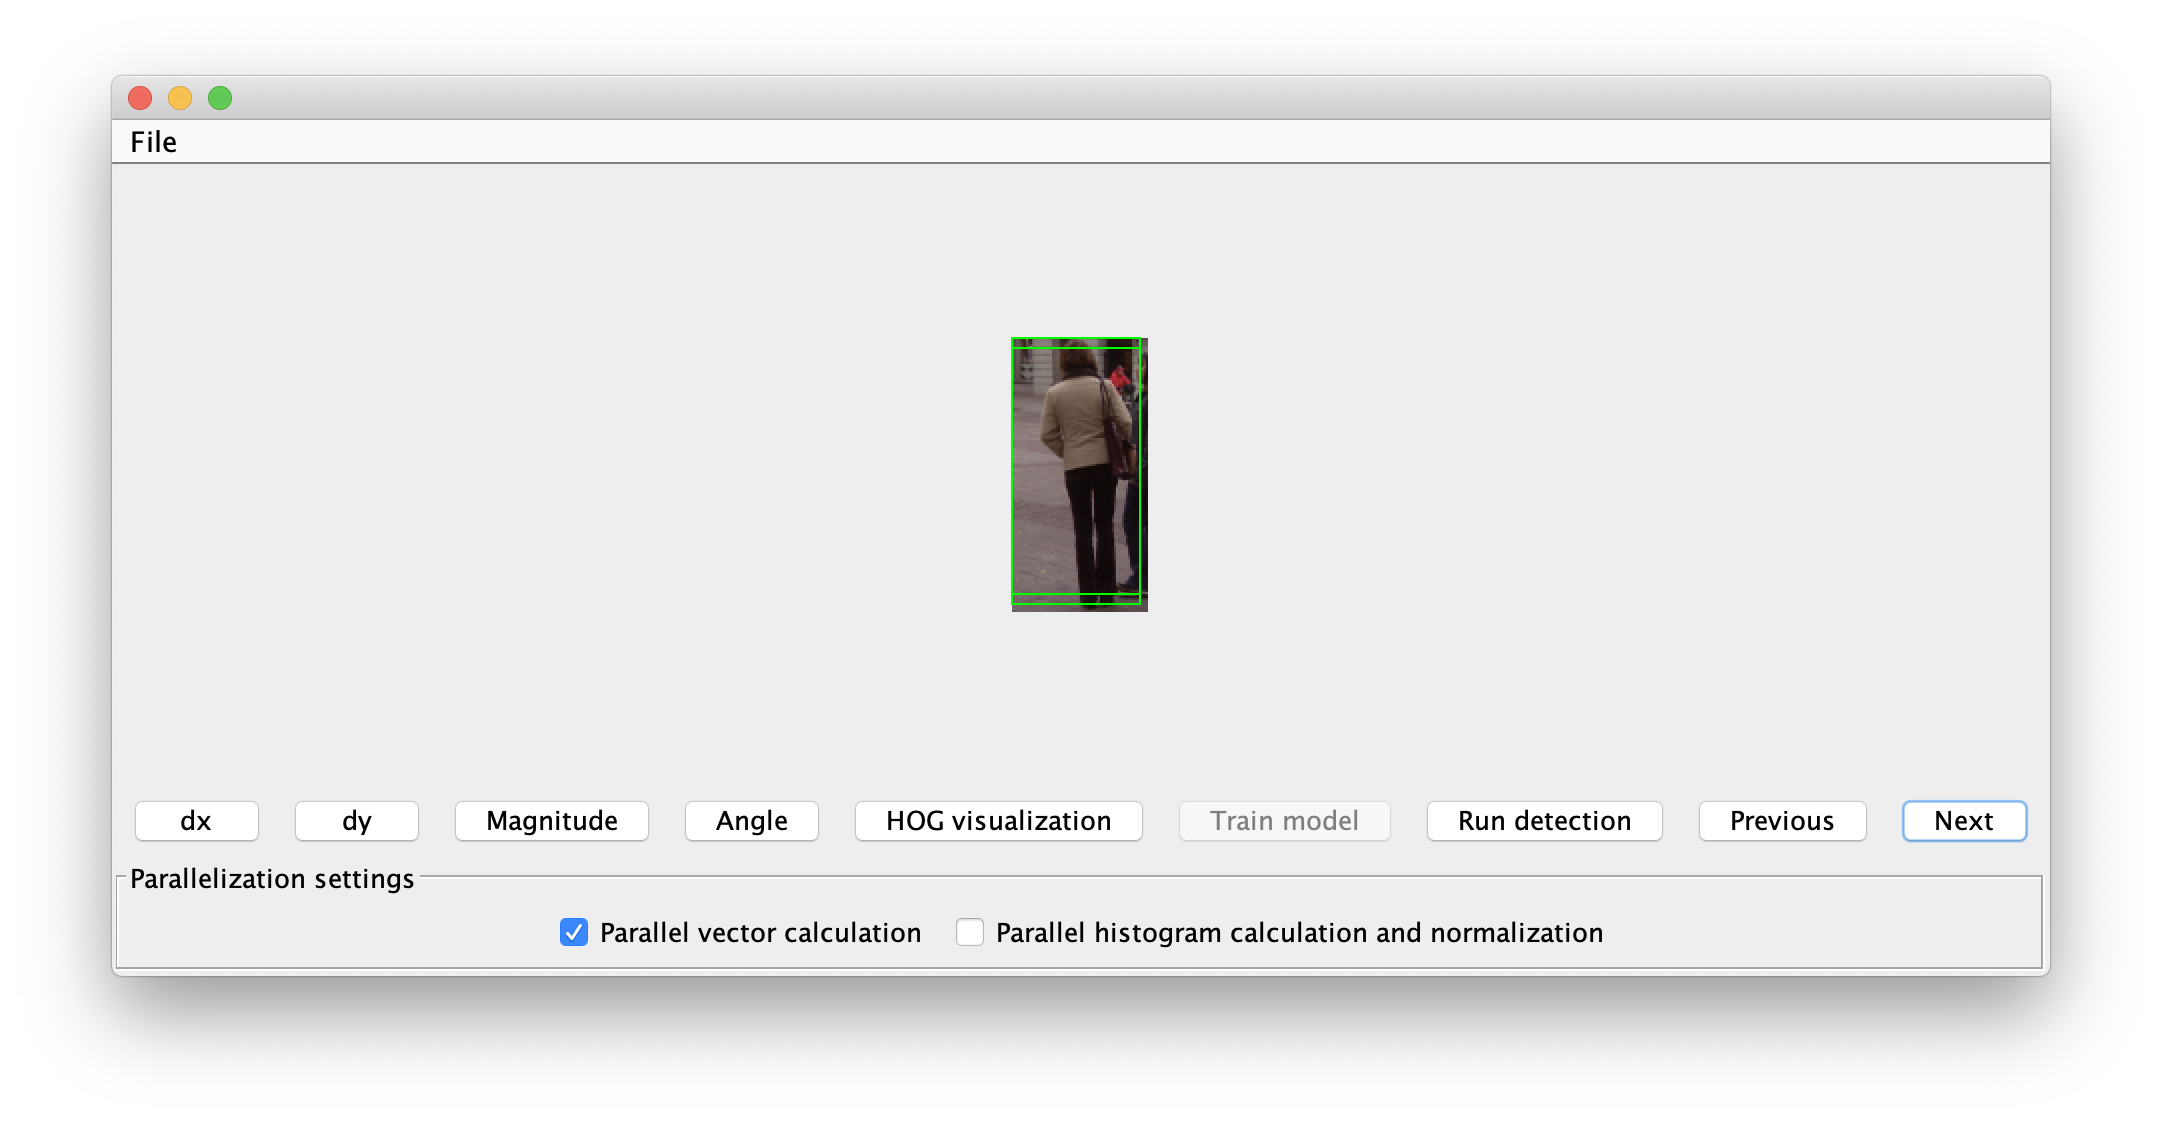
\includegraphics[width=\linewidth]{figures/scaledDetection.png}
	\caption{Detekcija pješaka na skaliranoj slici}
	\label{fig:scaledDetection}
\end{figure}

\chapter{Rezultati}
Najvažnija karakteristika algoritma u ovom radu, naravno osim točnosti, je brzina. U nastavku je dana usporedbe vremena izvođenja. Za svaku vrijednost mjerenje je ponovljeno 5 puta te su prosjek i standardna devijacija izračunati pomoću programskog jezika R. Vremena u tablicama iskazana su u sekundama. \\

Operacija računanja derivacije u smjeru \(x\) ili \(y\)-osi može se usporediti s operacijom filtriranja slike. Iz tog razloga u tablicama su dana mjerenja izvedbe Javine nativne operacije filtriranja.

\begin{table}[htb]
	\centering
	\caption{Izračun derivacije u smjeru \(x\)-osi}
	\label{tbl:dx}
	\begin{tabular}{llll} \hline
		Dimenzije & Java dx & Paralelizirani dx & dx\\ \hline
		64x128 & 0.0005$\pm$3.04e-5 & 0.0022$\pm$0.0005 & 0.0008$\pm$0.0004\\
		900x900 & 0.0204$\pm$0.0015 & 0.0109$\pm$0.0012 & 0.0204$\pm$0.0047\\
		1280x720 & 0.0207$\pm$0.0015 & 0.0131$\pm$0.002 & 0.0236$\pm$0.0043\\
		1000x2000 & 0.0431$\pm$0.0027 & 0.0284$\pm$0.0095 & 0.0406$\pm$0.0104\\ \hline
	\end{tabular}
\end{table}

Iz tablice~\ref{tbl:dx} vidljivo je da jednodretvena izvedba u prosijeku radi jednako dobro kao i Javina nativna implementacija, ali uz veću standardnu devijaciju. Višedretvena izvedba radi brže od jednodretvene i nativne za slike velikih dimenzija, ali za male slike pokazalo se da je jednodretvena izvedba puno brža.

\chapter{Zaključak}
Zaključak.

\bibliography{literatura}
\bibliographystyle{fer}

\begin{sazetak}
Sažetak na hrvatskom jeziku.

\kljucnerijeci{Ključne riječi, odvojene zarezima.}
\end{sazetak}

\engtitle{Multi-threaded Implementation of Algorithm for Calculation of Histogram of Oriented Gradients in Images}
\begin{abstract}
Abstract.

\keywords{Keywords.}
\end{abstract}

\end{document}
